\documentclass[12pt, a4paper, UTF8]{article}
\usepackage{ctex}
\usepackage{indentfirst}
\usepackage{amsmath}
\usepackage{amsfonts}
\usepackage{amssymb}
\usepackage{graphicx}
\usepackage{geometry}
\usepackage{booktabs}
\usepackage{caption}
\usepackage{subcaption}
\usepackage{hyperref}
\usepackage{siunitx}
\usepackage{enumitem}
\usepackage{xeCJK}
\usepackage{array}
\usepackage{listings}
\usepackage{xcolor}
\usepackage{epstopdf}
\usepackage{float} % [H] 固定浮动体位置

\hypersetup{hidelinks}

\title{实验报告：7nm FinFET 器件几何结构校准}
\author{作者：徐子翔 \hspace{0.2cm} 郦查德}
\date{\today}

\begin{document}

\maketitle

\section{实验目的}
本次实验旨在利用 GTS TCAD 仿真平台，基于 7nm n型体硅 FinFET的图像，完成器件几何结构的初步校准。通过调节 Structure 模块中的物理参数，使仿真生成的 3D 模型与实际工艺形貌相匹配，为后续的电学性能仿真奠定几何基础。

\section{实验内容与操作步骤}

\subsection{环境搭建与版图导入}
\begin{enumerate}
    \item 将模板项目 \texttt{N7\_TEM\_Calibration} 拷贝至工作目录。
    \item 在 Structure 模块中打开路径下的 N7 版图文件。
    \item 执行 \texttt{Create device} 生成初始三维结构并观察各组件空间关系。
\end{enumerate}


\subsection{Fin Profile 校准}
\begin{enumerate}
    \item Fin Width 校准：fin width对应active fin底部的宽度，从图中给的两个fin对应的宽度后取平均值。
    \item Sub Fin 高度校准（srbHeight）：在两个sub fin之间最低处画水平切线作为基准，量取其到分界线的长度，按照比例尺等比例缩放得到实际的 sub fin 高度。
    \item Active Fin 校准(finHeight)：量取分界线之间的长度，按照比例尺等比例缩放得到实际的 active fin 高度。
    \item Active Fin倾角（finTopTaperingDeg）与Sub Fin 倾角(srbBottomTaperingDeg)校准：根据截面图，绘制与4个侧面相切的斜边，量取4个倾角后取平均值作为 active fin 与 sub fin 的倾角。
    \item 栅金属高度（contactThickness）校准：按照比例尺可测得contactThickness = 13.75nm。
    \item 栅氧化层（IL 层与 HighK 层）厚度暂设为默认值。
\end{enumerate}

\begin{figure}[H]
    \centering
    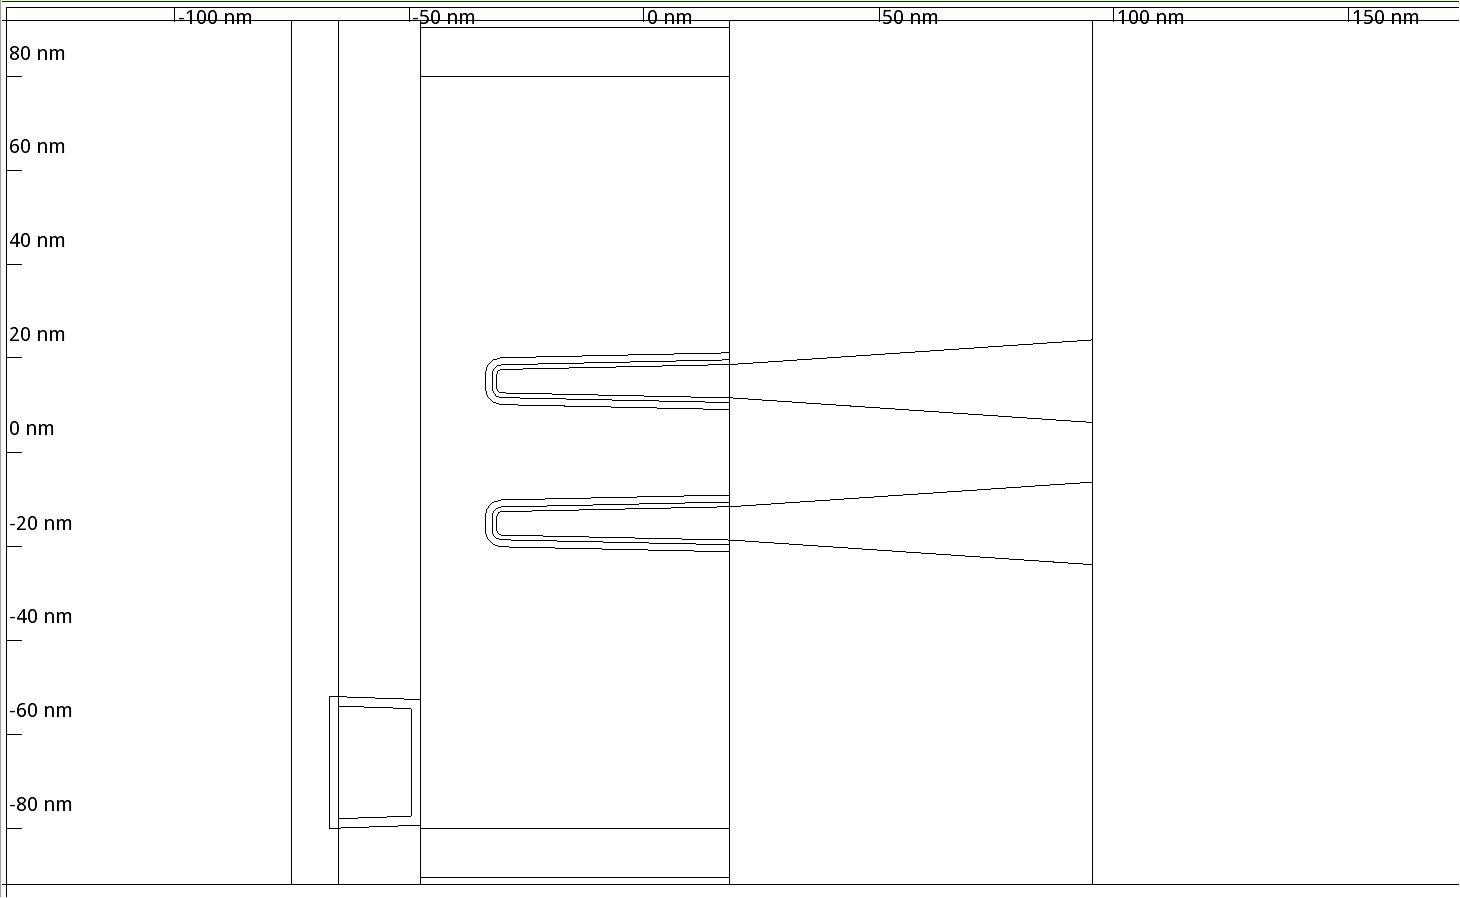
\includegraphics[width=0.8\linewidth]{images/2.2.png}
    \caption{Fin Profile 截面图}
    \label{fig:fin-2-2}
\end{figure}

\begin{figure}[H]
    \centering
    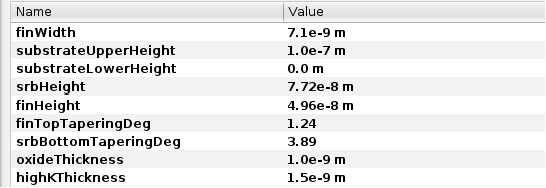
\includegraphics[width=0.8\linewidth]{images/2.2parameter.png}
    \caption{Fin Profile 参数}
    \label{fig:fin-2-2-param}
\end{figure}

\subsection{Epi（源漏外延）形貌校准}
根据GtsTechX-Manual，GTS用epiGrowExtraTop和epiGrowExtraBottom描述Epi的位置和大小，用epiAspectRatio（即宽长比）描述Epi的形状。

epiGrowExtraTop=epiGrowExtraBottom=0时，Epi的位置和大小如图~\ref{fig:epi_manual}所示。

\begin{figure}[htbp]
    \centering
    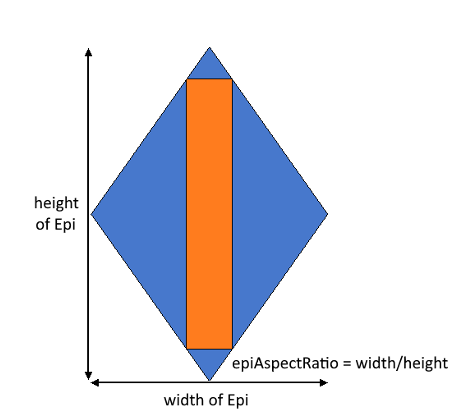
\includegraphics[width=0.7\textwidth]{images/epi_manual.png}
    \caption{Epi位置和大小示意图}
    \label{fig:epi_manual}
\end{figure}

Epi对应的菱形切过一个矩形，其宽为finWidth，上下两条宽的位置分别位于Active Fin的上表面和下表面。
epiGrowExtraTop和epiGrowExtraBottom分别表示矩形上面那条宽向上平移的距离和下面那条宽向下平移的距离。

\begin{enumerate}
    \item epiGrowExtraTop和epiGrowExtraBottom校准
    
        从TEM图中可以看出epiGrowExtraTop = 0nm，epiGrowExtraBottom = -12nm。
    \item epiOuterClipDistanceSide和epiAspectRatio校准
    
        将TEM图导入ImageJ，并绘制辅助线，如图~\ref{fig:epi_and_CT}所示。

        \begin{figure}[htbp]
            \centering
            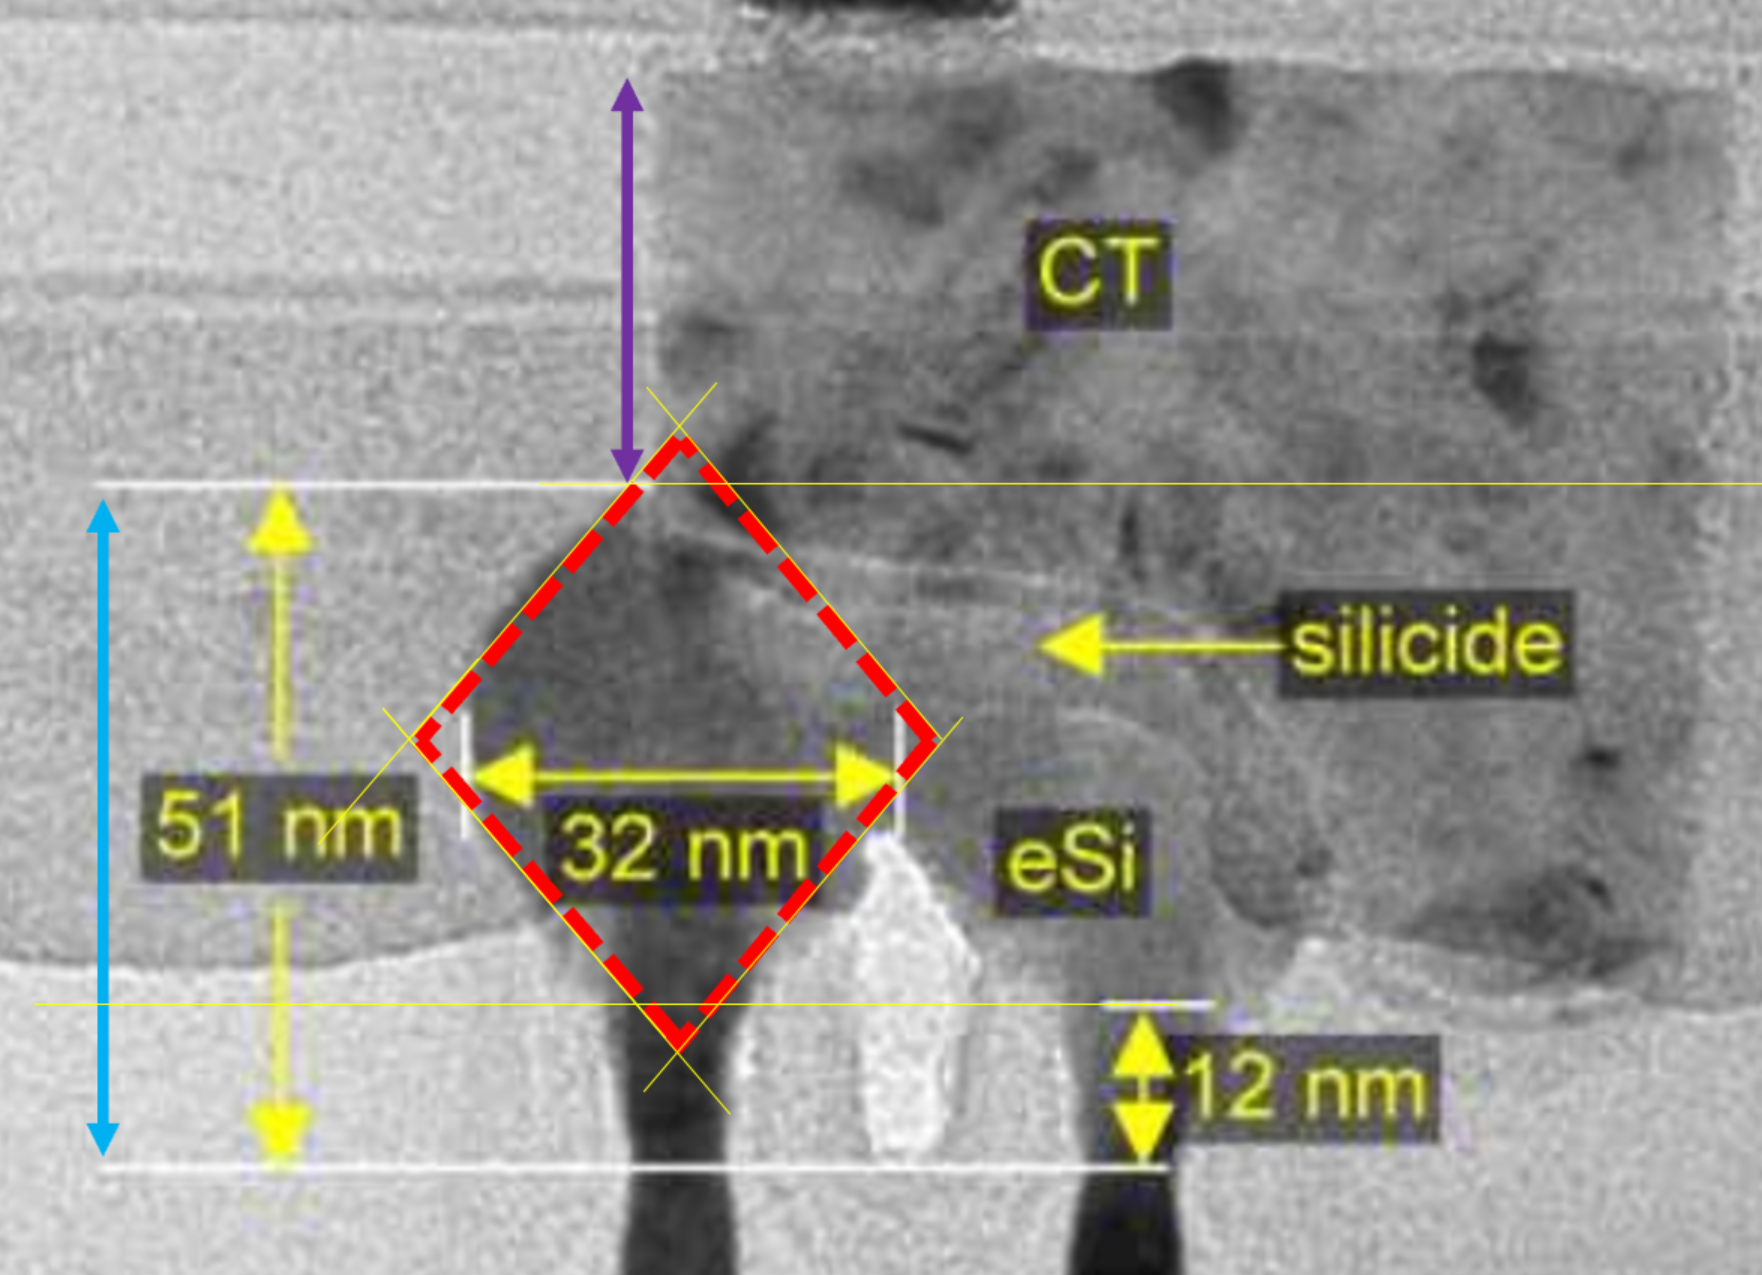
\includegraphics[width=0.8\textwidth]{images/epi_and_CT.png}
            \caption{TEM图导入ImageJ}
            \label{fig:epi_and_CT}
        \end{figure}

        以51nm为基准，可测量出菱形长度为47.44nm，宽度为39.99nm，Epi宽度为32.36nm。由此可计算出：

        \[\text{epiAspectRatio}=\frac{\text{菱形宽度}}{\text{菱形长度}}=0.843\]

        \[\text{epiOuterClipDistanceSide}=\frac{\text{菱形宽度}-\text{Epi宽度}}{2}=3.81\si{nm}\]

    \item epiOuterClipDistanceTop校准
    
        从图中直接量的话可能会有较大误差，这里借助GTS来完成。

        现在GTS中设置epiOuterClipDistanceTop为0，create device之后测量出Epi上顶点到Active Fin底部的距离，再与51nm作差，即得到需要切掉的长度。

        用此方法可以得到epiOuterClipDistanceTop=3.21nm。

    \item epiOuterClipDistanceBottom校准
    
        由于Epi底部和Fin融合，这个参数可设为0。
\end{enumerate}

\subsection{金属形貌校准}
\begin{enumerate}
    \item CT侧壁倾角（ContactAngleDeg）和contactBottomBarrierThickness校准
    
        可从图~\ref{fig:epi_and_CT}中直接测量出：
    
        ContactAngleDeg = 0，contactBottomBarrierThickness = 1.33nm。

    \item CT高度校准
    
        从图~\ref{fig:epi_and_CT}中可测量出CT高度=31.18nm。

        structure中没有直接与CT高度对应的参数，需要通过调节metal0Thickness来校准。

        校准方式类似epiOuterClipDistanceTop：先采用默认值，create device后测量出相应的CT高度，再与31.18nm做差，就得到了metal0Thickness需要变化的值。

        用此方法可以得到metal0Thickness = 15.86nm。

\end{enumerate}

\subsection{Gate Spacer 初步校准}
\begin{itemize}
    \item 根据已经校准的栅节距 $CGP=57\,\mathrm{nm}$、金属栅（MG）的物理栅长 $L_{\mathrm{phys}}=20\,\mathrm{nm}$ 和 CT 宽度 $=16\,\mathrm{nm}$，通过公式计算 Gate Spacer 厚度：
    \[
            \text{spacerLengthN}=\frac{CGP - MG - CT}{2}
    \]
\end{itemize}

\begin{figure}[H]
    \centering
    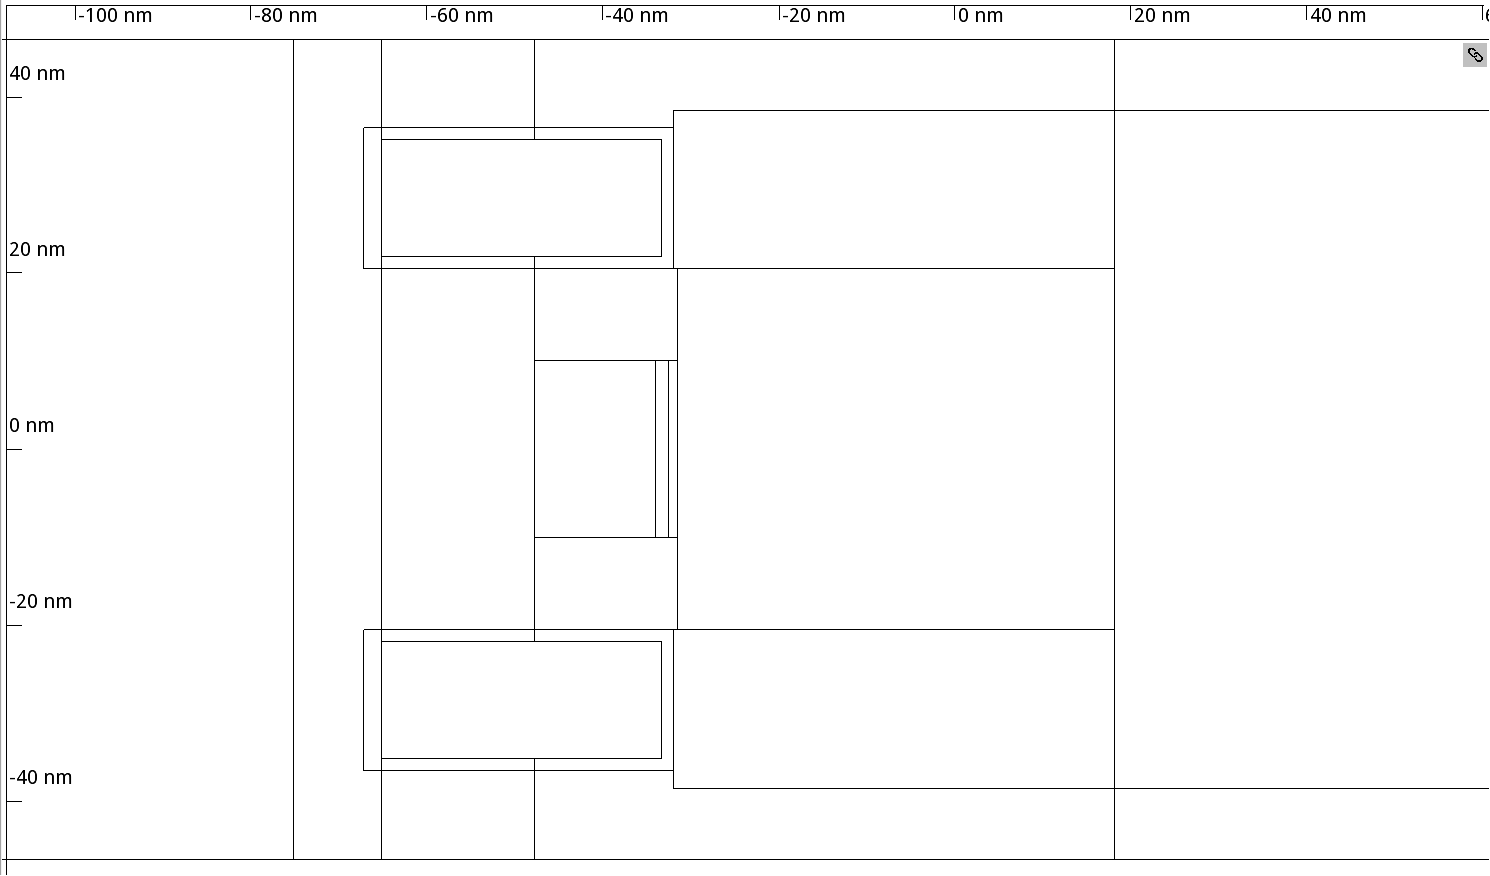
\includegraphics[width=0.8\linewidth]{images/2.5.png}
    \caption{Gate Spacer 截面图}
    \label{fig:gs-2-5}
\end{figure}

\begin{figure}[H]
    \centering
    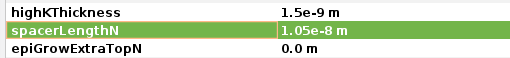
\includegraphics[width=0.8\linewidth]{images/2.5parameter.png}
    \caption{Gate Spacer 参数}
    \label{fig:gs-2-5-param}
\end{figure}

\section{总结}
本实验完成了 7nm n型 FinFET 的几何建模与初步校准。通过逐项调节 Fin 的高度与侧壁倾角、Epi 外延层的宽度与菱形倾角、CT的高度以及gate spacer的宽度，仿真模型在主要几何特征（高度、宽度、倾角）上已与 TEM 参考图达到良好一致。

已将最终确定的一套几何参数保存为 ipds 文件，以便复现与后续电学仿真使用。形貌误差的主要来源还有 IL/HighK 薄层厚度的测量不确定性，因此后续需通过 IV/CV 特性拟合来精调这些薄层参数以进一步提升模型的准确性。

总之，本次几何校准为后续电学性能仿真与器件优化提供了可重复的基础模型和初始参数集，为下一步进行电学仿真与性能分析奠定了坚实的基础。

\end{document}